\section{Results and Analysis}


\subsection{Effects of number of clients on FOLtR-ES}
%To answer RQ1, we perform experiments on MLSR-WEB10K dataset with the same FOLtR-ES setup
%Reproducing FOLtR-ES on other datasets

To study the influence of number of clients, we perform experiments on MQ2007 and MSLR-WEB10K datasets. 

\begin{figure}[H]
	\centering
	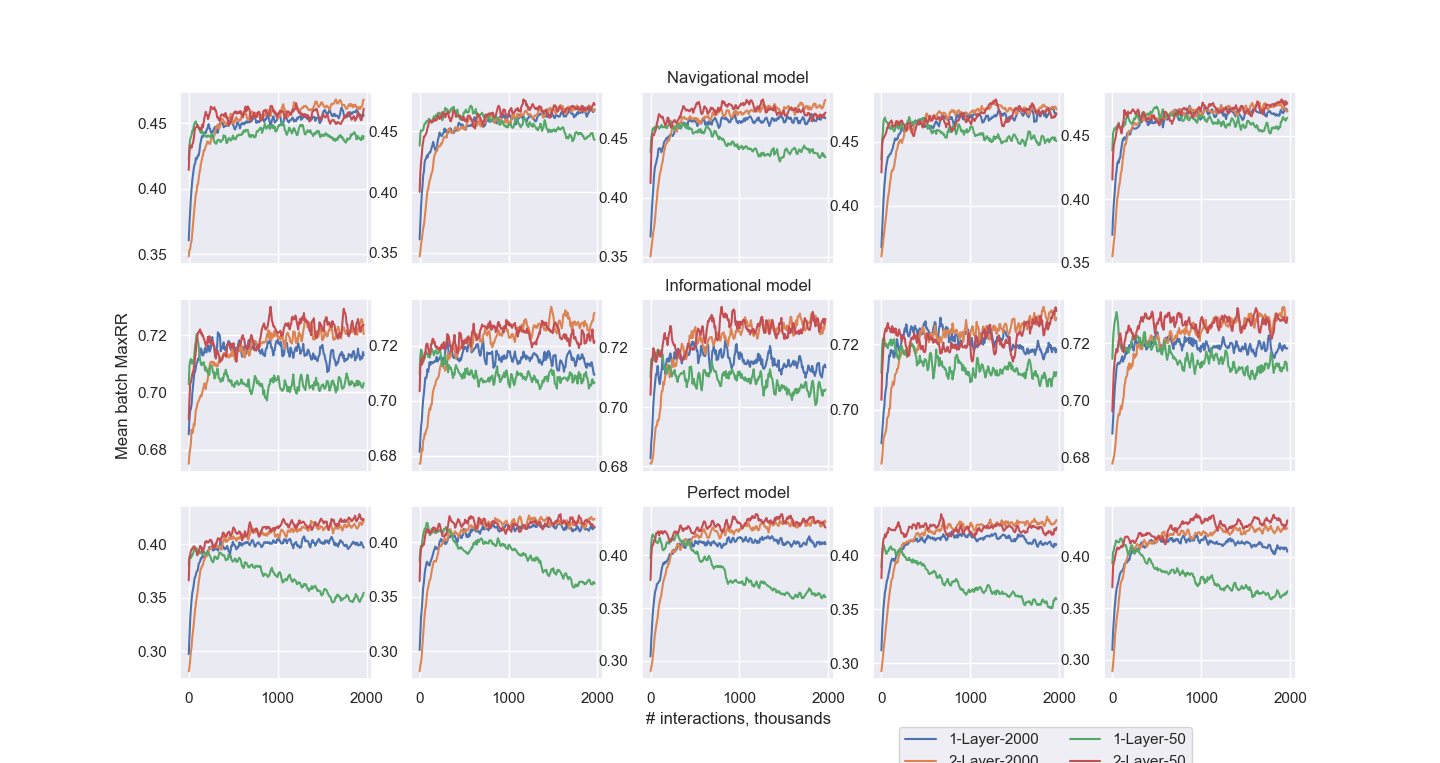
\includegraphics[width=16cm, height=8cm]{v0_mq2007_foltr_clients_p0.9.png}
	\caption{Mean batch MaxRR for MQ2007 with different client number}
	\label{fig: mq2007clients}
\end{figure}


\subsection{Comparing FOLtR-ES with OLTR baselines}

For a fair comparation, we set up the privacy probability $p = 1$ (lowest privacy) in FOLtR-ES. We perform experiments on MQ2007 and MLSR-WEB10K datasets with simulating 2000 clients.

\begin{figure}[H]
	\centering
	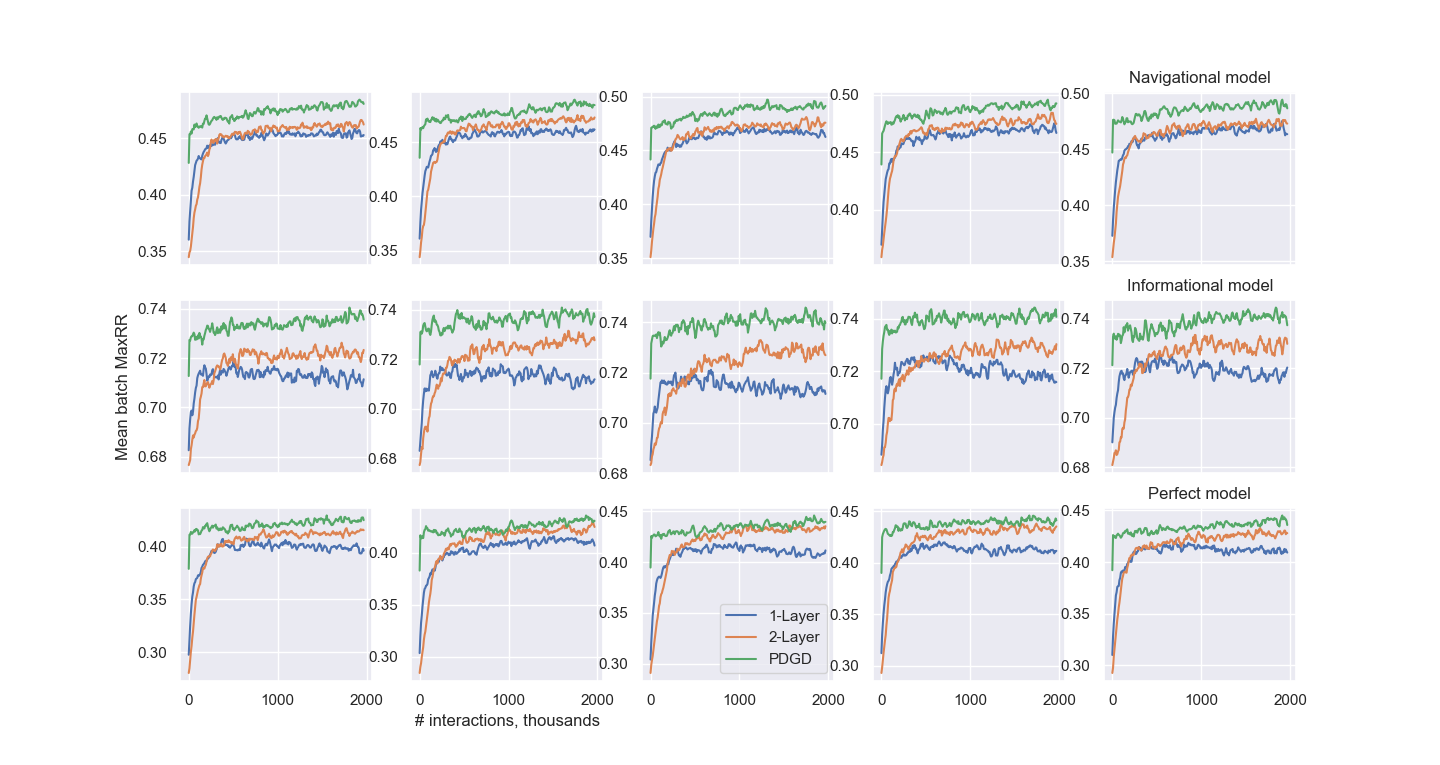
\includegraphics[width=16cm, height=8cm]{v0_mq2007_foltr_vs_pdgd_2000clients_p1.0.png}
	\caption{Mean batch MaxRR for MQ2007 with 2000 clients and $p = 1$}
	\label{fig: mq2007-v0}
\end{figure}

\begin{figure}[H]
	\centering
	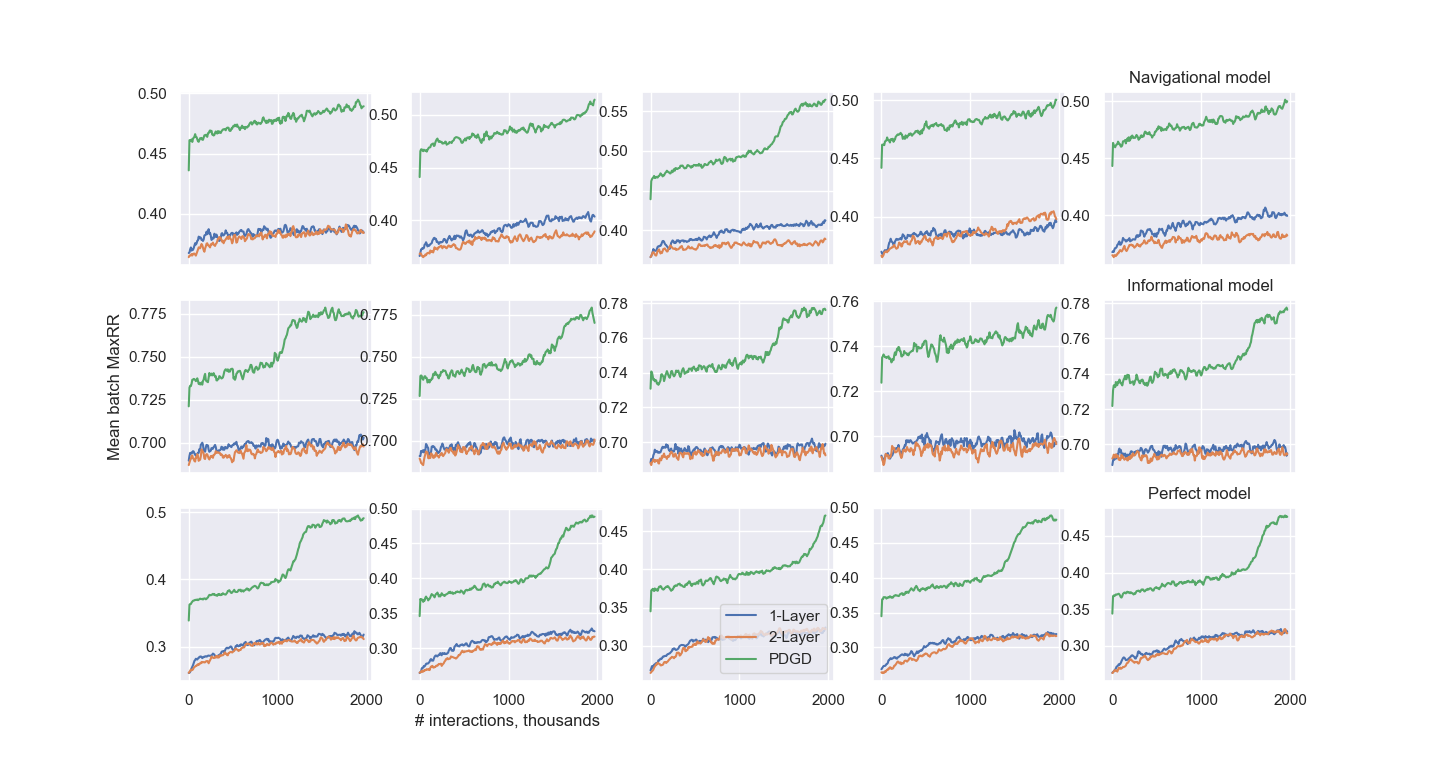
\includegraphics[width=16cm, height=8cm]{v0_mslr_foltr_vs_pdgd_2000clients_p1.0.png}
	\caption{Mean batch MaxRR for MSLR-WEB10K with 2000 clients and $p = 1$}
	\label{fig: mslr-v0}
\end{figure}

